%\section{Objectifs de la vérification formelle}


%enjeux de sécurité du projet (produit de sécurité = wookey)
%reprendre des exemples des pres du SSTIC

\section{Prise en main de Frama-C}

\subsection{Installation}

L'installation de la plateforme Frama-C (version 20.0 Calcium) a été réalisée à l'aide du gestionnaire de packet opam, qui permet d'avoir un environnement compatible avec l'utilisation de Frama-C. Pour compléter l'installation de Frama-C, des prouveurs externes ont également été installés, dans leur dernière version à l'exception d'Alt-ergo :
\begin{itemize}
	\item Alt-ergo version 2.3.0\footnote{la dernière version est la 2.3.2, mais il est conseillé d'utiliser la version 2.3.0 pour des raisons de compatibilité avec why3, la plateforme exécutant les différents solveurs externes},
	\item CVC4 version 1.7
	\item Z3 version 4.8.6
\end{itemize}

\subsection{Tutorial}

La première partie du stage a consisté à prendre en main Frama-C, les greffons EVA et WP ainsi qu'à apprendre les bases du langage ACSL. À ce titre, j'ai suivi plusieurs tutoriels :
\begin{itemize}
	\item pour WP et ACSL, j'ai suivi un tutoriel en ligne (\url{https://zestedesavoir.com/tutoriels/885/introduction-a-la-preuve-de-programmes-c-avec-frama-c-et-son-greffon-wp}) détaillant l'utilisation de WP mais présentant également de nombreux exercices sur des contrats de fonction simples, réalisés en ACSL. De plus, le manuel en référence XX (ACSL by Example) présente de nombreux exemples de complexité croissante permettant de prendre en main ACSL et de monter en compétence.
	\item Pour EVA, j'ai suivi un tutoriel en ligne (\url{http://blog.frama-c.com/index.php?post/2017/03/07/A-simple-EVA-tutorial}) ainsi que le tutoriel présenté dans le manuel d'EVA (référence XX). Ces tutoriels expliquent la prise en main du greffon EVA sur des exemples simples, donnent quelques conseils génériques d'analyse et présentent notamment l'utilisation de l'interface graphique avec EVA,
\end{itemize}

\noindent En complément de ces différents tutoriels, chaque greffon de Frama-C dispose d'un manuel utilisateur (XX et XX) présentant la plupart des options pouvant être utilisées avec les greffons. Toutefois, les exemples donnés ne sont pas toujours bien illustrés, et toutes les options ne sont pas présentes. Il est ainsi nécessaire de se référer à l'aide en ligne de commande, installée en même temps que Frama-C.

\section{Utilisation de Frama-C sur la bibliothèque USBctrl}

La stratégie suivie pour l'analyse de la bibliothèque USBctrl avec Frama-C a été présentée dans le chapitre \ref{strategie}. Elle comporte 3 étapes, détaillées dans les paragraphes ci-dessous:
\begin{itemize}
	\item Parsing du code source de la bibliothèque USBctrl,
	\item Analyse avec EVA,
	\item Analyse avec WP.
\end{itemize}


\subsection{Parsing du code source de la bibliothèque USBctrl de WooKey}

La première étape de l'analyse de la bibliothèque USBctrl a consisté à vérifier que Frama-C pouvait parcourir l'ensemble des fichiers de la bibliothèque ainsi que ceux utilisés par la bibliothèque (fichiers du driver, fichiers de configuration...). Frama-C a été utlisée avec la ligne de commande suivante :
\begin{lstlisting}[style=CStyle]
frama-c usbctrl.c usbctrl_descriptors.c usbctrl_handlers.c usbctrl_requests.c
 usbctrl_state.c framac/include/driver_api/usbotghs_frama.c -c11
 -machdep x86_32 -no-frama-c-stdlib -cpp-extra-args="-nostdinc -I framac/include"
\end{lstlisting}

\noindent Cette ligne de commandes est constituée :
\begin{itemize}
	\item des fichiers qui seront analysés par Frama-C : les 5 fichiers de la bibliothèque USBctrl et 1 fichier d'un driver USB \footnote{Le driver high speed codé dans WooKey se compose de 4 fichiers, pour des raisons pratiques j'ai choisi de concaténer ces différents fichiers dans un seul fichier, ce qui n'a aucune conséquence sur l'analyse réalisée avec Frama-C}
	\item d'options :
		\begin{itemize}
			\item c11 car la bibliothèque USBctrl comporte du code utilisant le standard ANSI c11. Il est nécessaire de préciser cette option car, nativement, Frama-C utilise les standards c90 et c99. Sans cette option, Frama-C ne peut donc pas analyser du code C écrit dans le standard c11,
			\item machdep x86\_32 afin d'indiquer à Frama-C que la machine sur laquelle est censée s'exécuter le code est une machine 32 bits (l'architecture de WooKey est une architecture 32 bits),
			\item no-frama-c-stdlib pour indiquer à Frama-C de ne pas utiliser la bibliothèque standard du C généralement installée sur toutes les distributions Linux. En effet, WooKey dispose de sa propre version de cette bibliothèque,
			\item cpp-extra-args="-nostdinc -I framac/include", afin d'indiquer à Frama-C dans quel répertoire se trouvent les fichiers nécessaires pour compiler les fichiers analysés (bibliothèque C de WooKey, fichiers de configuration...).
		\end{itemize}
\end{itemize}

\subsection{Utilisation d'EVA}

Une fois le parsing des fichiers réalisé avec Frama-C, la deuxième étape a consisté à utiliser EVA.

\subsubsection{Stratégie d'analyse}

L'analyse des fichiers avec EVA nécessite un point d'entrée dans le code source, à partir duquel EVA peut analyser les différentes fonctions du code source. Par défaut, ce point d'entrée est la fonction main du code analysé, mais ce n'est pas obligatoire et il est possible de définir n'importe quelle fonction comme point d'entrée en précisant cette fonction dans les options d'EVA. Une fois un point d'entrée dans le code défini, l'analyse avec EVA peut être effectuée. Deux critères sont importants pour estimer la pertinence de l'analyse réalisée:
\begin{itemize}
	\item le taux de couverture du code analysé
	\item la précision de l'analyse réalisée
\end{itemize}

\noindent L'objectif est d'obtenir un taux de couverture du code maximal, avec la meilleure précision possible. De cette manière, il est possible de garantir à l'absence de RTE avec EVA, pour des expressions simples, car EVA réalise une analyse correcte \footnote{La notion de correction est définie dans le chapitre \ref{chapitre_1}. Cela signifie que l'analyse d'EVA ne comporte pas de faux négatifs, toutes les erreurs potentielles sont détectées }. La figure suivante représente l'objectif recherché de l'analyse réalisée avec EVA:

\begin{figure}[!h]
\centering
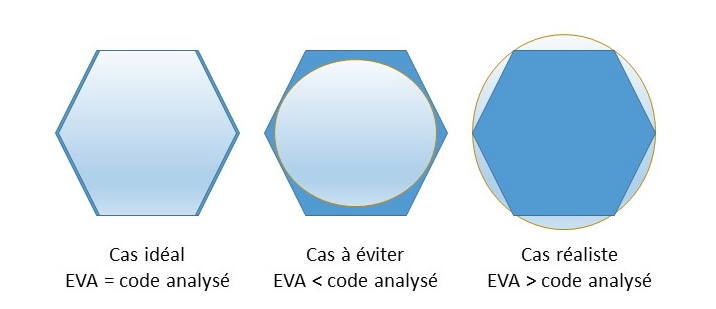
\includegraphics[width=16cm]{images/schema_analyse_eva.png}
\caption{Schéma d'analyse avec EVA}
\label{Schéma d'analyse avec EVA}
\end{figure}

\noindent Le premier cas représente le cas idéal: l'interprétation abstraire d'EVA correspond exactement au code source analysé.
\newline \noindent Dans le deuxième cas, le taux de couverture du code analysé n'est pas suffisant, et l'interprétation abstraite d'EVA ne permet pas de couvrir tout le code. Il existe donc des parties du code qui ne sont pas analysées par EVA, et il n'est donc pas possible de conclure à l'absence de RTE (même si EVA est correct).
\newline \noindent Enfin, dans le dernier cas, qui correspond à l'objectif visé, le taux de couverture du code est suffisant et l'interprétation d'EVA réalise une sur-approximation du code analysé. Combiné au caractère correct d'EVA, il est possible dans ce cas de conclure à l'absence d'erreur dans le code analysé.
%revoir: ce n'est pas totalement absence d'erreur
\newline
\newline \noindent Le taux de couverture du code analysé est indiqué dans le résumé de l'analyse d'EVA, comme illustré dans la figure suivante:

\begin{figure}[!h]
\centering
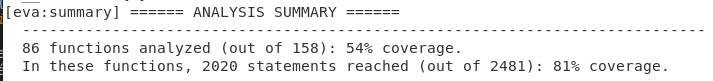
\includegraphics[width=10cm]{images/taux_couverture_eva.png}
\caption{Taux de couverture - EVA}
\label{Taux de couverture - EVA}
\end{figure}

\noindent Dans cet exemple, 54\% de l'ensemble des fonctions du code source sont analysés : 86 fonctions sur 158, en incluant l'ensemble des fichiers inclus, qui ne sont pas forcément à analyser). Le taux de couverture des fonctions analysés est alors de 81\% dans cet exemple. Le taux de couverture global du code doit donc s'évaluer à partir du nombre de fonctions analysées, et de leur couverture. Par exemple, si une seule fonction est analysée parmis une quarantaine de fonction, même si elle est analysée à 100\%, le taux de couverture sera faible. De même, si 100\% des fonctions sont analysés mais le taux de couverture de ces fonctions ne dépasse pas 10\%, cela signifie qu'EVA n'analyse quasiment pas ces fonctions, même si EVA y rentre.
\newpage \noindent Par ailleurs, le taux de couverture du code peut être vérifié à l'aide de l'interface graphique de Frama-C, comme le montre la figure suivante:


\begin{figure}[!h]
\centering
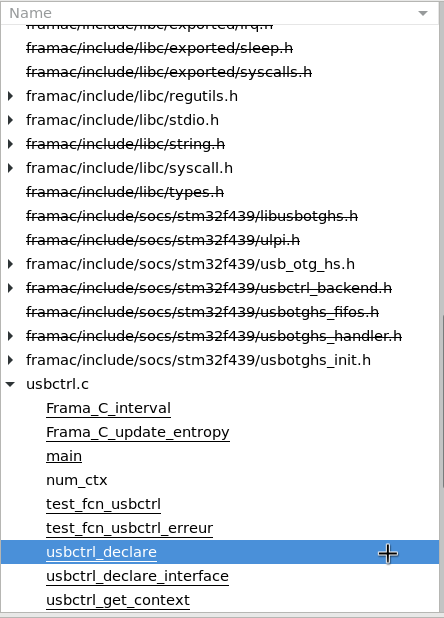
\includegraphics[width=8cm]{images/taux_couverture_eva_GUI.png}
\caption{Visualisation des fichiers analysés avec EVA - Interface graphique}
\label{Visualisation des fichiers analysés avec EVA - Interface graphique}
\end{figure}

\noindent Sur cette figure, les fichiers et fonctions que Frama-C peut analyser sont indiqués sur la partie gauche. Les fonctions et fichiers non analysés par EVA sont barrés.

\newpage \noindent
De plus, il est possible de visualiser pour une fonction donnée sa couverture dans l'onglet principal, comme illustré dans la figure suivante:

\begin{figure}[!h]
\centering
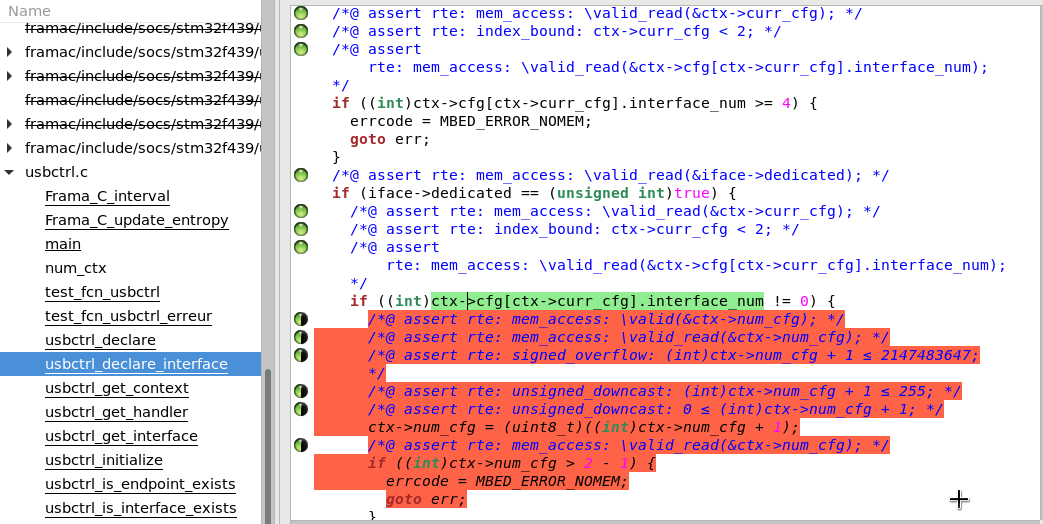
\includegraphics[width=16cm]{images/taux_couverture_eva_GUI_fonction.png}
\caption{Fonction analysée avec EVA - Interface graphique}
\label{Fonction analysée avec EVA - Interface graphique}
\end{figure}


\noindent Dans cet exemple, le contexte d'appel de la fonction analysée, usbctrl\_declare\_interface, ne permet pas d'entrer dans une structure conditionnelle. Pour augmenter le taux de couverture, il faut modifier le point d'entrée de l'analyse avec EVA en ajoutant les fonctions manquantes et en jouant sur les paramètres d'entrées afin par exemple de parcourir l'ensemble des embranchements possibles dans une fonction et en incluant les cas d'erreur le cas échéant.

%%%%%%%%%%%%%%%%%%%%%%%%%%%%%%%%%%%%%%%%%%%%
%%%%%%%%%%%%%%%%%%%%%%%%%%%%%%%%%%%%%%%%%%%%

\newpage \noindent Le deuxième paramètre important pour l'analyse avec EVA est la précision de l'analyse. En effet, si l'interprétation réalisée avec EVA n'est pas suffisament précise, il ne sera pas possible d'obtenir l'ensemble des valeurs possibles pour toutes les variables du code analysé, et par conséquent il ne sera pas possible de conclure en l'absence d'erreur. En contrepartie, une plus grande précision sous-entend une durée de calcul plus importante.
\newline \noindent La précision de l'analyse est paramétrable à travers les options d'EVA, notamment 2 options:
\begin{itemize}
	\item eva-auto-loop-unroll n\footnote{n entier positif} : cette option permet à EVA d'analyser les boucles (boucles for, boucles while), n représentant le nombre maximum d'itérations dans les boucles. Sans cette option, ou avec un n trop faible, il n'est pas possible à EVA de dérouler complètement les boucles présentes dans le code. Par conséquent, pour certaines itérations, l'interprétation réalisée par EVA ne sera pas suffisament précise pour déterminer le comportement de la boucle et les valeurs prises par les variables dans la boucle.
	\item eva-slevel n\footnote{n entier positif} : l'utilisation de cette option permet à EVA de garantir la précision de l'interprétation abstraire, en particulier pour les fonctions présentant des boucles ou des structures conditionnelles. Le slevel peut être vu comme un "carburant" donné à EVA, consommé en parcourant une fonction en présence de boucles et de structures conditionnelles\footnote{l'utilisation de cette fonction rend de fait optionnelle l'utilisation de loop unroll}. En l'absence de "carburant" ou avec une quantité trop faible, EVA n'est pas capable de séparer l'ensemble des états possibles dans une fonction, et réalise une fusion de ces états. Par conséquent, il n'est pas possible à EVA de déterminer dans ce cas l'ensemble des valeurs possibles pour les différentes variables de cette fonction. Cette option, notamment quand le slevel est élevé, augmente fortement le temps de l'analyse. Pour réduire ce temps, tout en conservant la précision de l'analyse, il est possible d'utiliser l'option suivante -eva-slevel-function fcn:n afin de personnaliser le slevel pour une fonction donnée. Il est ainsi possible d'augmenter le slevel pour les fonctions le nécessitant, et de prendre un slevel plus faible pour les autres fonctions\footnote{le slevel-function est considéré à la place du slevel général}.
\end{itemize}

\noindent L'analyse des logs permet de vérifier la précision de l'analyse réalisée avec EVA. En effet, la présence du mot clé "merge" indique des imprécisions. Il est ainsi possible d'augmenter pour l'ensemble du code le slevel jusqu'à sa disparition, ou de ne l'augmenter que pour certaines fonctions.

\subsubsection{options d'utilisation de FRAMAC}\label{optionsEVA}

L'analyse avec EVA est réalisée en lançant la commande suivante :

\begin{lstlisting}[style=CStyle]
	frama-c usbctrl.c usbctrl_descriptors.c usbctrl_handlers.c
	usbctrl_requests.c usbctrl_state.c framac/include/driver_api/usbotghs_frama.c \
			-c11 -machdep x86_32 \
	        -no-frama-c-stdlib \
	        -warn-left-shift-negative \
	        -warn-right-shift-negative \
	        -warn-signed-downcast \
	        -warn-signed-overflow \
	        -warn-unsigned-downcast \
	        -warn-unsigned-overflow \
			-kernel-msg-key pp \
			-cpp-extra-args="-nostdinc -I framac/include" \
		    -rte \
		    -eva \
		    -eva-warn-undefined-pointer-comparison none \
		    -eva-auto-loop-unroll 500 \
		    -eva-slevel 500 \
		    -eva-slevel-function usbctrl_get_descriptor:12000 \
		    -eva-slevel-function usbotghs_send_data:1000 \
		    -eva-slevel-function usbotghs_endpoint_stall:1000 \
		    -eva-slevel-function usbotghs_endpoint_set_nak:1000 \
		    -eva-symbolic-locations-domain \
		    -eva-equality-domain \
		    -eva-bitwise-domain \
		    -eva-equality-through-calls-function usbctrl_start_device \
		    -eva-equality-through-calls-function usbctrl_is_valid_transition \
  			-wp-dynamic \
		    -eva-split-return auto \
		    -eva-partition-history 3 \
		    -eva-use-spec class_get_descriptor \
		    -eva-use-spec usbctrl_reset_received \
		    -eva-log a:frama-c-rte-eva.log \
			-save framac/results/frama-c-rte-eva.session
\end{lstlisting}

Cette ligne de commandes est constituée :
\begin{itemize}
	\item d'options pour le noyau de Frama-C (depuis -c11 jusqu'à -rte) :
		\begin{itemize}
			\item des options nécessaires pour le parsing du code source, explicitées dans le paragraphe précédant
			\item absolute-valid-range 0x40040000-0x400150000, afin d'indiquer à Frama-C que les adresses mémoires situées entre 0x40040000 et 0x400150000 sont valides. Cette plage d'adresse représente, pour le driver USB High Speed, les adresses mémoires du périphérique dans lesquelles le driver peut accéder en lecture et en écriture. Cette plage d'adresse est dépendante du driver USB utilisé et doit donc être modifiée en cas d'utilisation d'analyse d'un autre driver USB. Cette option est nécessaire car ces adresses ne sont pas allouées lors de l'exécution de la bibliothèque USBctrl, mais sont écrites dans un fichier source. Il fallait donc indiquer à Frama-C que ces adresses représentaient des adresses mémoires valides, accessibles en lecture et en écriture
			\item des options afin de vérifier que le code ne contient pas d'overflow sur des entiers signés ou non signés, ou que des downcast d'entiers signés ou non signés ne sont pas réalisés par le code (les downcast et les overflow d'entiers sont des sources de RTE) (options préfixées par -warn)
			\item l'option -rte permet à EVA et à WP d'annoter automatiquement le code avec des assertions ACSL, visualisables avec l'interface graphique (le code source n'est pas modifié). Cela permet de voir les assertions prouvées ou non par EVA, par exemple. La figure suivante illustre des assertions automatiques , prouvées et non prouvées par EVA:

\begin{figure}[!h]
\centering
%\includegraphics[width=16cm]{images/illustration_rte_GUI.png}
\caption{Visualisation des annotations automatiques avec l'interface graphique}
\label{Visualisation des annotations automatiques avec l'interface graphique}
\end{figure}

			Dans cet exemple...blablabla


		\end{itemize}
	\item des options pour le greffon EVA, identifiées par le prefixe -eva :
		\begin{itemize}
			\item eva-warn-undefined-pointer-comparison none : cette option permet de désactiver la verification pour les comparaisons de pointeurs (très bof, à revoir...)
			\item des options pour la précision de l'analyse : -eva-auto-loop-unroll, -eva-slevel et -eva-slevel-function (voir si plevel utile...)
			\item eva-symbolic-locations-domain, -eva-bitwise-domain et -eva-equality-domain :
			\item eva-split-return auto : pour avoir des états séparés à la fin de chaque fonction, afin d'avoir une analyse plus précise
			\item eva-partition-history 3 : permet d'analyser avec précision les fonctions comportant de nombreuses structures conditionnelles (structures if/else, switch...)
			\item eva-use-spec fcn : permet d'indiquer à EVA de ne prendre en compte que le contrat de la fonction fcn et non le corps de la fonction. Utile quand la fonction n'est pas définie, par exemple (ce qui est le cas pour les fonctions class\_get\_descriptor et usbctrl\_reset\_received).
		\end{itemize}
\end{itemize}

\noindent Des options sont par ailleurs activées par défaut, en particulier l'option -wp-dynamic qui pour utiliser des annotations spécifiques pour les pointeurs de fonction. Cela permet à EVA d'analyser correctement les pointeurs de fonctions, en parcourant la fonction "pointée". Des annotations spécifiques sont toutefois nécessaires, comme le montre l'exemple suivant :
\newline \noindent /*@ assert fcn {\&fcn1} ; */
\newline \noindent /*@ calls fcn1; */


%-warn-left-shift-negative can be used to check that the code does not perform signed left shifts on negative values, i.e., x << n with x having signed type and negative value. This is set by default, and can be disabled with option -no-warn-left-shift-negative
%-warn-right-shift-negative, as its left-shift counterpart, can be used to check for nega- tive right shifts, i.e., x >> n with x having signed type and negative value. This is not set by default. -no-warn-right-shift-negative can be used to disable the option if previously enabled.

%-warn-signed-downcast may be used to check that the analyzed code does not downcast an integer to a signed integer type. This option is not set by default. Without it, the analyzers do not perform such a verification. For instance consider the following function.
%short truncate( int n) {
%return (short) n;
%}

% If -warn-signed-downcast is set, analyzers report an error on ( short ) n which downcasts a signed integer to a signed short. Without it, no error is reported.
% -warn-unsigned-downcast is the same as -warn-signed-downcast for downcasts to unsigned integers. This option is also not set by default.

% -warn-signed-overflow may be used to check that the analyzed code does not overflow on integer operations. If the opposite option -no-warn-signed-overflow is specified, the analyzers assume that operations over signed integers may overflow by following two’s complement representation. This option is set by default. For instance, consider the function abs that computes the absolute value of its int argument.
% int abs(int x) {
% if (x < 0) x = -x;
% return x;
% }
% By default, analyzers detect an error on -x since this operation overflows when MININT is the argument of the function. But, with the -no-warn-signed-overflow option, no error is detected.
% -warn-unsigned-overflow is the same as -warn-signed-overflow for operations over unsigned integers. This option is not set by default.


\subsection{Utilisation de WP}

La 3ème étape consiste à analyser le code avec WP, à la suite de l'analyse réalisée avec EVA. Comme expliqué dans le chapitre \ref{strategie}, cela permet à WP d'utiliser les résultats de l'analyse d'EVA afin notamment de prouver l'absence de RTE pour des cas plus complexes que ceux validés avec EVA.

\subsubsection{stratégie d'analyse}

Le greffon WP, contrairement au greffon EVA, ne nécessite pas de point d'entrée dans le code analysé. WP étant modulaire, l'analyse peut être réalisée fonction par fonction, après les avoir spécifiées avec un contrat de fonction écrit en ACSL (comme illustré dans le chapitre \ref{contrats}). L'objectif est d'obtenir pour l'ensemble des fonctions de la bibliothèques USBctrl une spécification validée par WP, comprenant des préconditions, des postconditions et des assigns, incluant le cas échéant des spécifications de boucles, afin de statuer sur l'absence de RTE et sur la bonne terminaison des fonctions.
\newline \noindent
La stratégie mise en place au cours de ce stage pour y parvenir a été la suivante:
\begin{itemize}
	\item établir le contrat des fonctions de la bibliothèque USBctrl indépendantes des autres fonctions de la bibliothèque ou du driver USB
	\item établir le contrat des fonctions du driver USB appelées par la bibliothèque USBctrl
	\item établir le contrat des fonctions de la bibliothèque USBctrl qui appèlent d'autres fonctions de la bibiothèque ou du driver USB.
\end{itemize}

Il est en effet nécessaire de commencer à spécifier les fonctions "appelées" avant de passer aux fonctions "appelantes" car le comportement des fonctions "appelantes" peut dépendre du résultat des fonctions "appelées".
\newline \noindent
Pour une fonction donnée, les spécifications se font en plusieurs étapes :
\begin{itemize}
	\item établissement des préconditions (assumes et requires) et des postconditions, celles-ci portant sur le résultat de la fonction (par exemple, un code d'erreur). Il s'agit de spécifier la fonction sans rentrer finement dans le détail de son comportement, afin de vérifier son comportement général.
	\item spécification des boucles présentes dans les fonctions. Comme expliqué dans le chapitre \ref{Boucles WP}, il s'agit, pour chaque boucle, de déterminer les propriétés valides avant d'entrer dans la boucle et qui le seront encore à la sortie de boucle (loop invariant), les variables modifiées par la boucle (loop assigns) et la propriété permettant de vérifier que la boucle se termine (loop variant)
	\item spécification des assigns dans les contrats de fonction, et ajout, le cas échéant, de post-conditions portant sur d'autres critères que la valeur de retour de la fonction en fonction de leur pertinence pour le comportement de la fonction. Par exemple, pour certaines fonctions modifiant l'état de la communication USB, il peut être pertinent de vérifier l'état atteint à la fin de la fonction. Cette dernière étape est la plus complexe, car elle nécessite d'une part d'identifier précisement les variables potentiellement modifiées par la fonction, mais également de comprendre quel était l'objectif recherché par la fonction, afin de déterminer des post-conditions représentatives de cet objectif.
\end{itemize}


\subsubsection{options d'utilisation de FRAMAC}\label{options pour WP}

L'analyse avec WP est réalisée en lançant la commande suivante :

\begin{lstlisting}[style=CStyle]
	frama-c usbctrl.c usbctrl_descriptors.c usbctrl_handlers.c
	usbctrl_requests.c usbctrl_state.c framac/include/driver_api/usbotghs_frama.c
			-c11 -machdep x86_32 \
	        -absolute-valid-range 0x40040000-0x400150000 \
	        -no-frama-c-stdlib \
	        -warn-left-shift-negative \
	        -warn-right-shift-negative \
	        -warn-signed-downcast \
	        -warn-signed-overflow \
	        -warn-unsigned-downcast \
	        -warn-unsigned-overflow \
			-kernel-msg-key pp \
			-cpp-extra-args="-nostdinc -I framac/include" \
		    -rte \
		    -eva \
		    -eva-warn-undefined-pointer-comparison none \
		    -eva-auto-loop-unroll 500 \
		    -eva-slevel 500 \
		    -eva-slevel-function usbctrl_get_descriptor:12000 \
		    -eva-slevel-function usbotghs_send_data:1000 \
		    -eva-slevel-function usbotghs_endpoint_stall:1000 \
		    -eva-slevel-function usbotghs_endpoint_set_nak:1000 \
		    -eva-symbolic-locations-domain \
		    -eva-equality-domain \
		    -eva-bitwise-domain \
		    -eva-equality-through-calls-function usbctrl_start_device \
		    -eva-equality-through-calls-function usbctrl_is_valid_transition \
		    -eva-split-return auto \
		    -eva-partition-history 10 \
		    -eva-use-spec class_get_descriptor \
		    -eva-use-spec usbctrl_reset_received \
		    -eva-log a:frama-c-rte-eva.log \
   		    -then \
   		    -wp \
  			-wp-model "Typed+ref+int" \
  			-wp-literals \
  			-wp-prover alt-ergo,cvc4,z3 \
   			-wp-timeout 15 \
   			-save $(SESSION) \
   			-time calcium_wp-eva.txt
\end{lstlisting}

Cette ligne de commande est consituée des options utilisées pour le parsing du code source et pour l'analyse avec EVA avec l'ajout des options suivantes :
\begin{itemize}
	\item -wp-model "Typed+ref+int" : cette option indique le modèle mémoire utilisé dans l'analyse WP:
		\begin{itemize}
			\item typed : dans ce modèle mémore, chaque pointeur déclaré dans le code analysé est considéré avec un type qui ne varie pas. Par exemple, si une variable est déclarée en tant que (uint\_8*), il ne sera pas possible de faire un cast vers un autre type de pointeur (WP ne sera pas capable dans ce cas de totalement valider les spécifications des fonctions dans lesquelles un tel cast serait fait)
			\item ref : %Activate the detection of pointer variables used for reference passing style.
			\item int : permet d'utiliser des entier de type machine (sur 32 bits par exemple) quand des overflows et ou des downcast peuvent se produire
		\end{itemize}
	\item -wp-literals : permet d'exporter le contenu des chaînes de caractères aux prouveurs (sans cette option, blabla)
	\item -wp-prover alt-ergo,cvc4,z3 : permet d'utiliser des prouveurs externes lors de l'analyse avec WP
	\item -wp-timeout 15 : indique à WP que chaque prouveur externe dispose de 15s pour valider une obligation de preuve, avant celle-ci ne soit considérée comme non prouvée
\end{itemize}





